\section{Results}
\label{sec:results}

\aim{Make similar plots for Brier (and CDE Loss?).}

\aim{Obviously this is too many plots!  Some can be condensed further, but there's a lot of redundancy.  For each ``dataset,'' I would like to show the different metrics' performance under each weighting.}

\subsection{Mock classifier systematics}
\label{sec:mockresults}

\begin{figure*}
	\begin{center}
		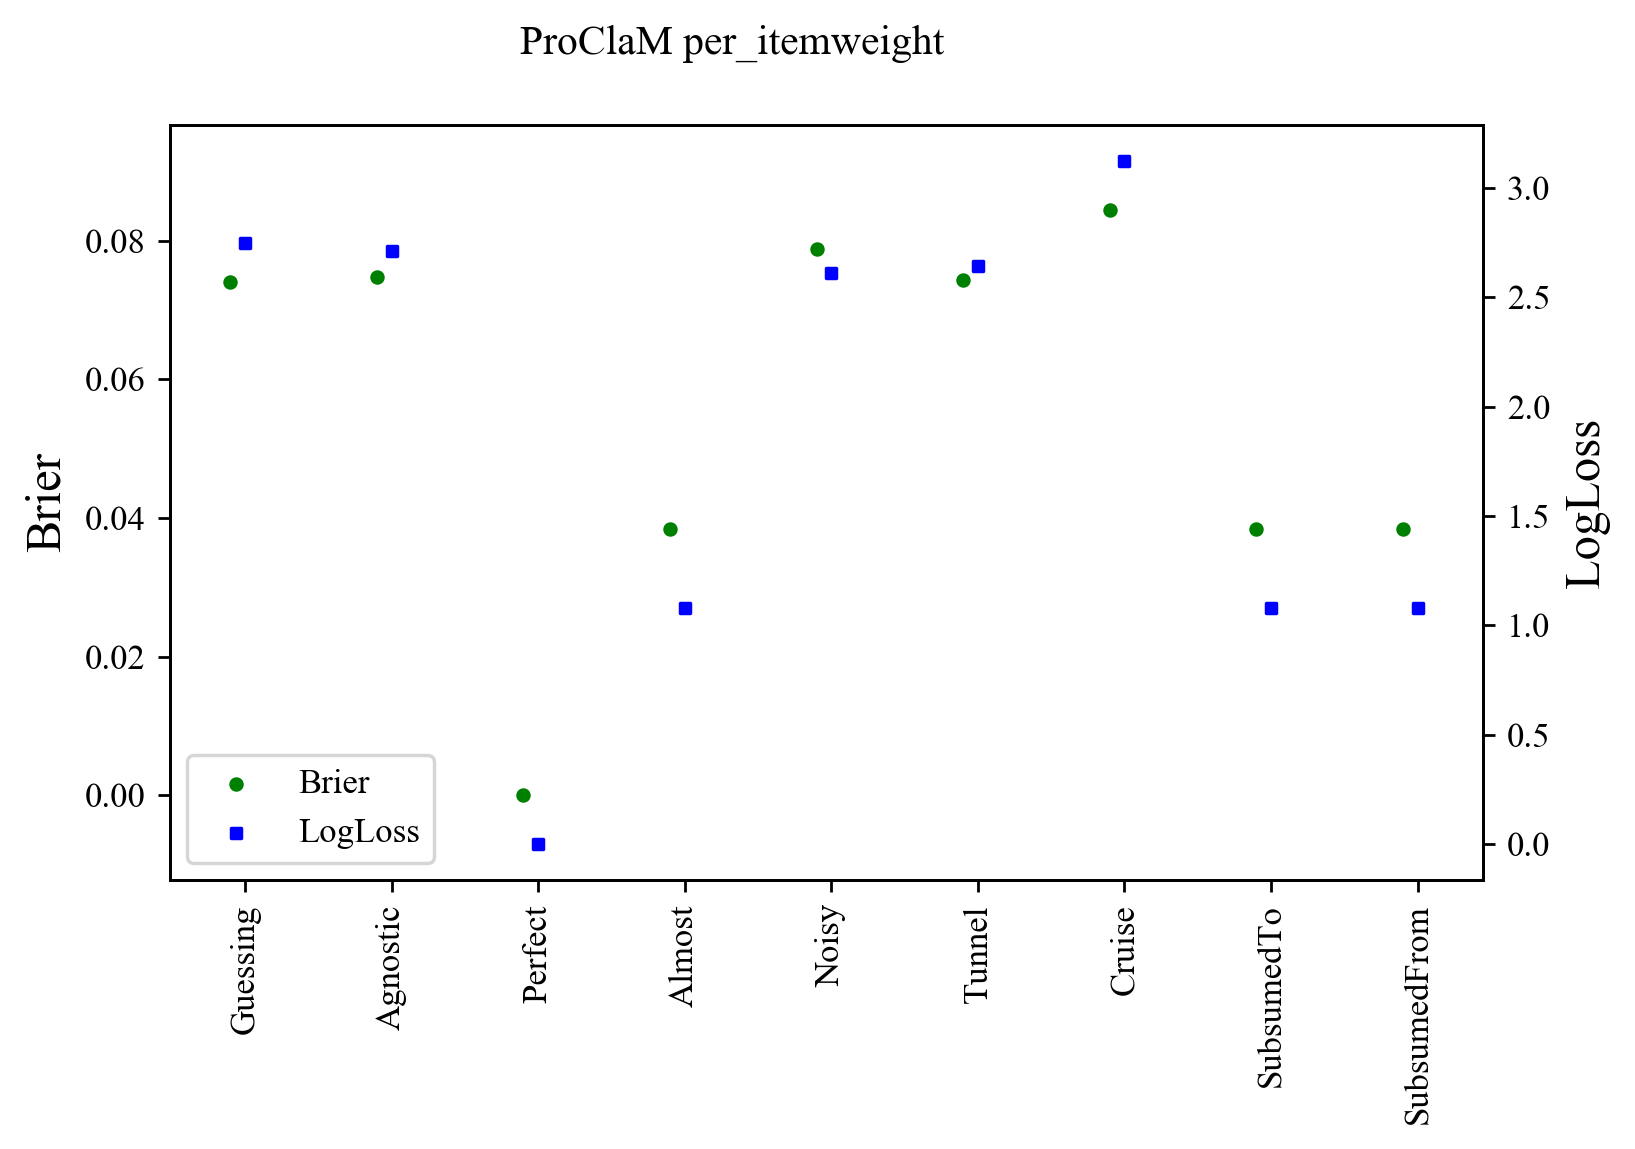
\includegraphics[width=0.45\textwidth]{./fig/multi_metric_per_item.png}
		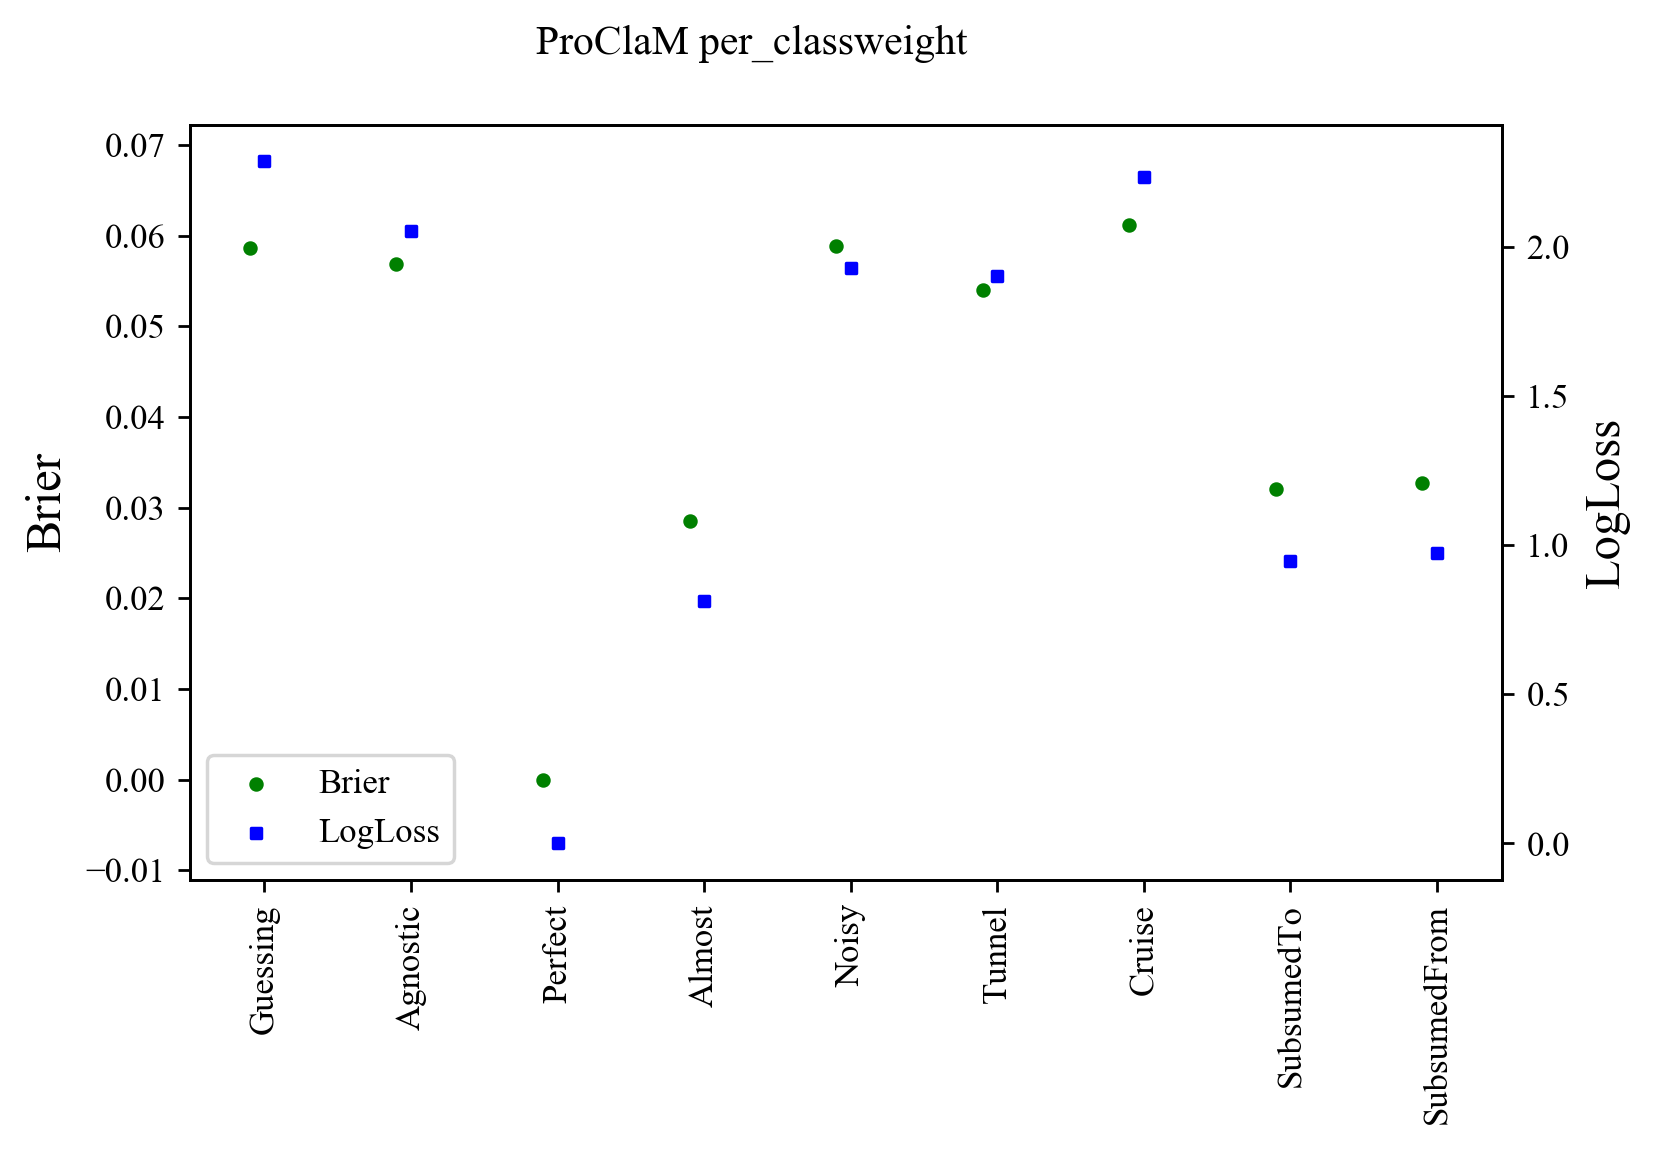
\includegraphics[width=0.45\textwidth]{./fig/multi_metric_per_class.png}
		\caption{left: equal weight per lightcurve, right: equal weight per class}
		\label{fig:fig:plasticc_per_item_vs_class}
	\end{center}
\end{figure*}

\begin{figure*}
	\begin{center}
		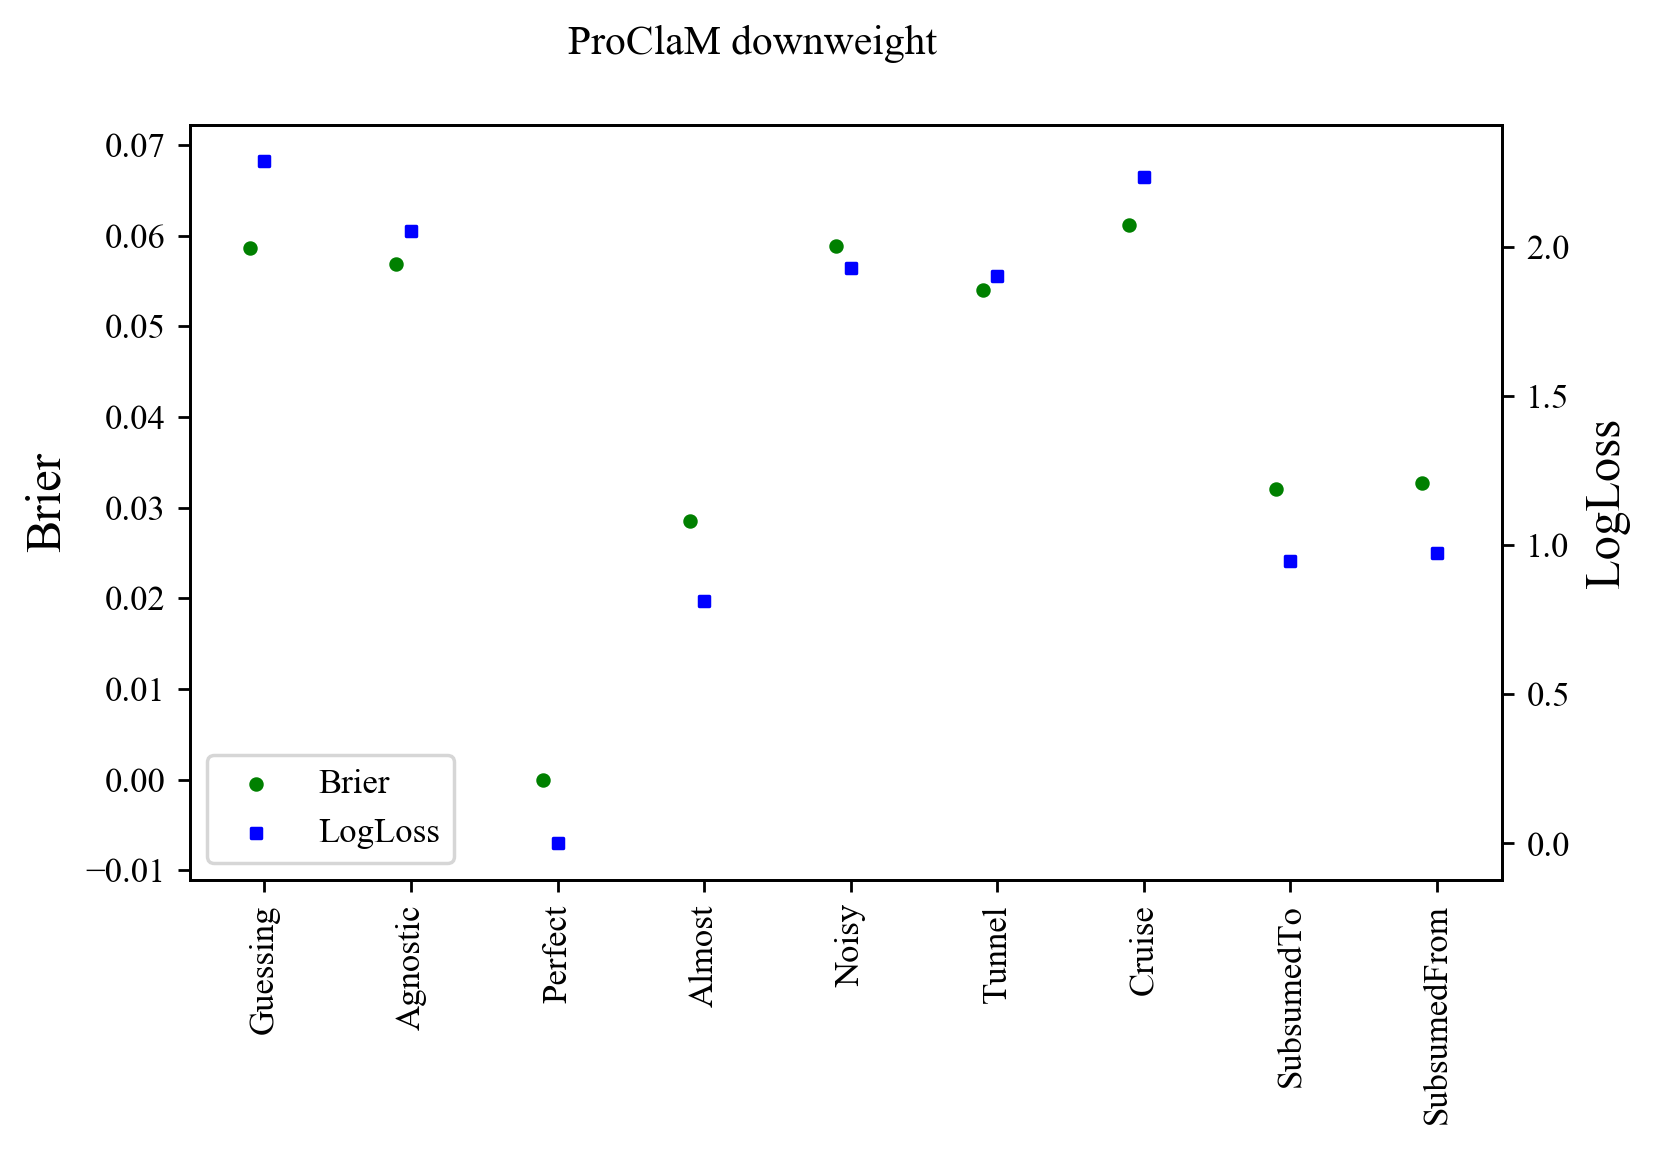
\includegraphics[width=0.45\textwidth]{./fig/multi_metric_down.png}
		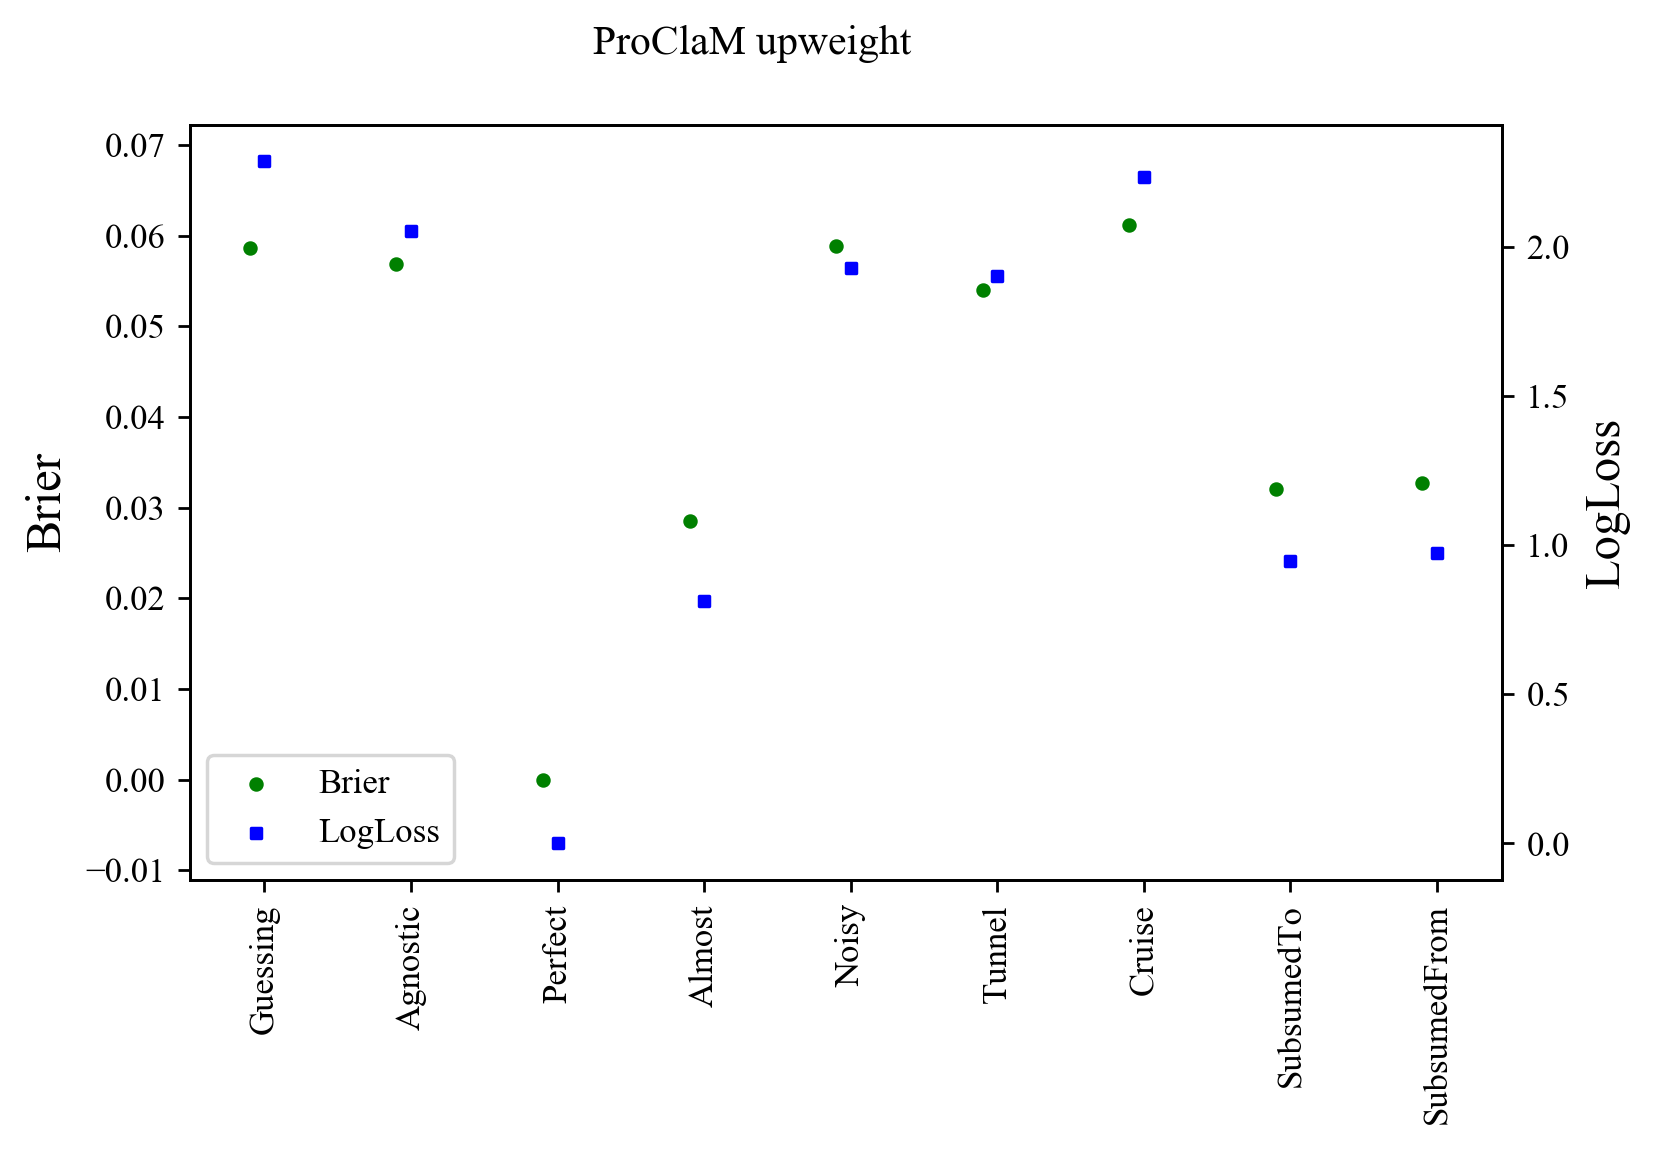
\includegraphics[width=0.45\textwidth]{./fig/multi_metric_up.png}
		\caption{left: downweight a particular class, right: upweight a particular class, \aim{This isn't interesting because the class is randomly chosen, might be more informative under per item weighting}}
		\label{fig:plasticc_down_vs_up_random}
	\end{center}
\end{figure*}


\subsection{Representative classifications}
\label{sec:realresults}

\begin{figure*}
	\begin{center}
		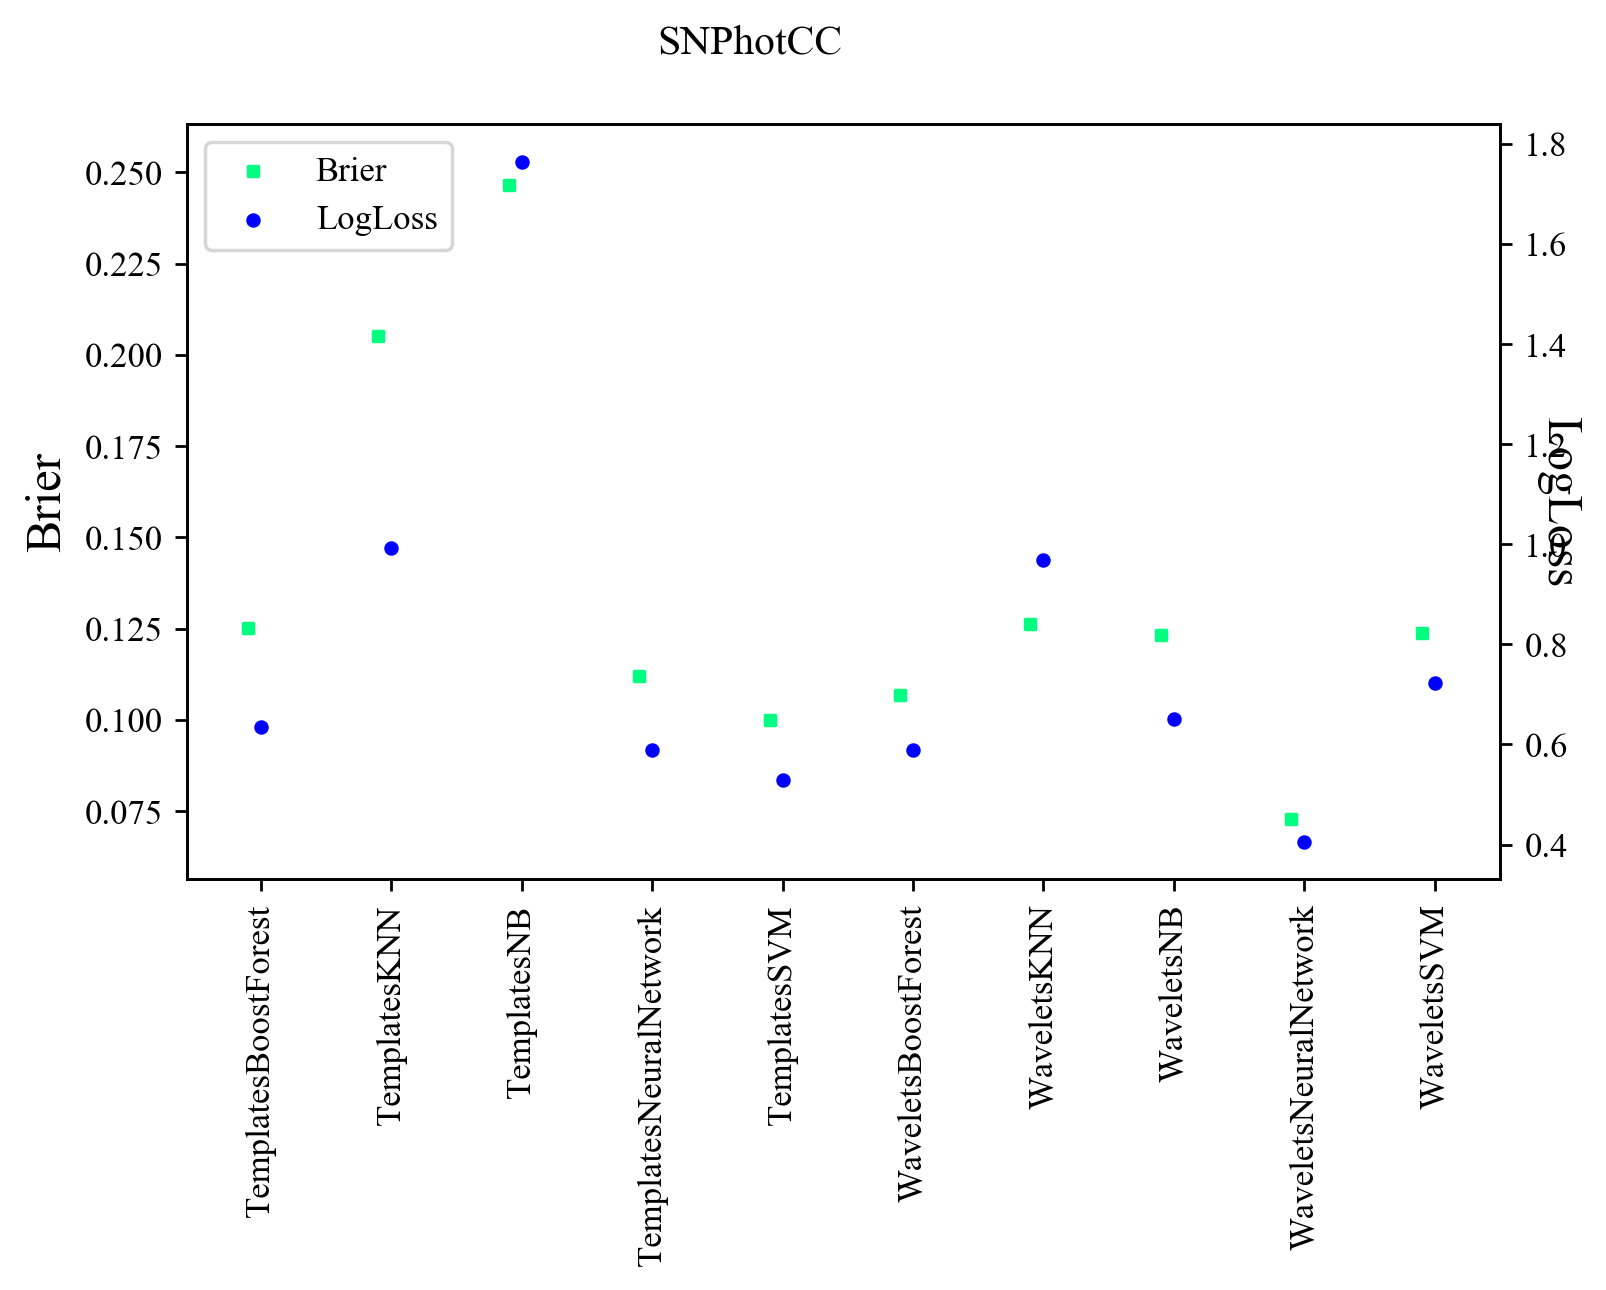
\includegraphics[width=0.45\textwidth]{./fig/SNPhotCC_res.png}
		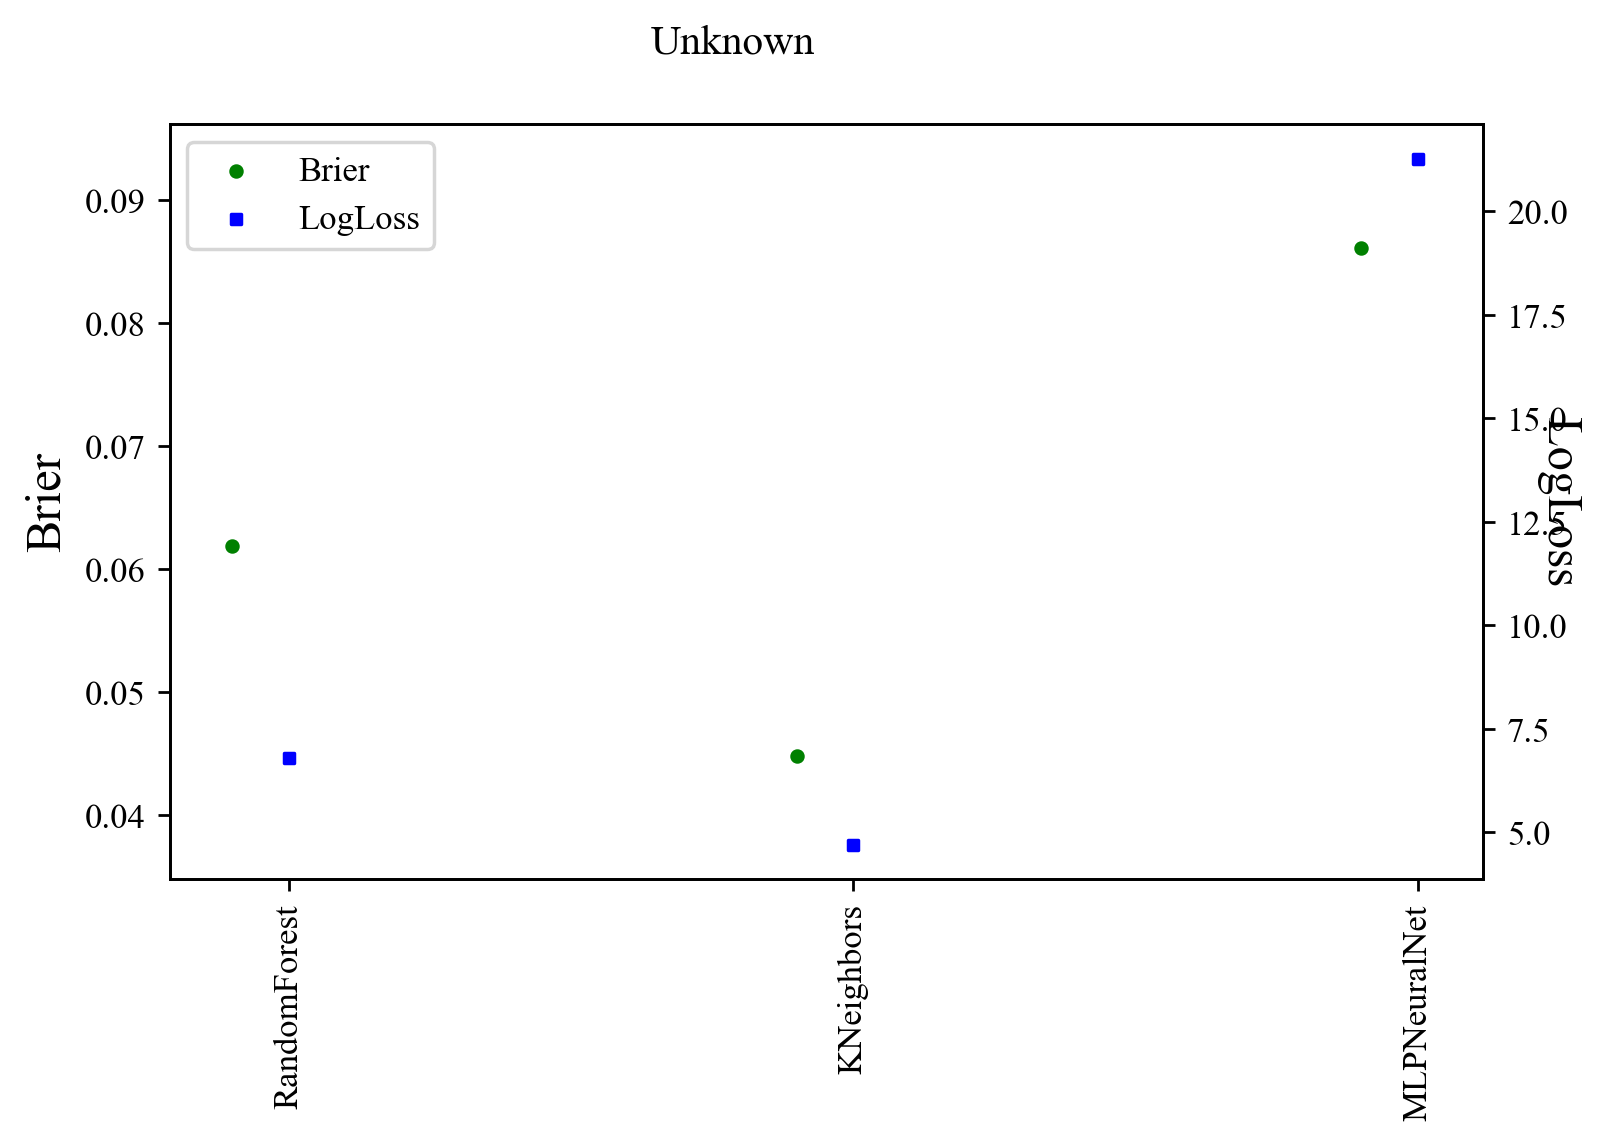
\includegraphics[width=0.45\textwidth]{./fig/Unknown_res.png}
		\caption{equal weight per class}
		\label{fig:real_metric_compare}
	\end{center}
\end{figure*}

\subsection{Weighting systematics}
\label{sec:weight_res}

\begin{figure}
	\begin{center}
		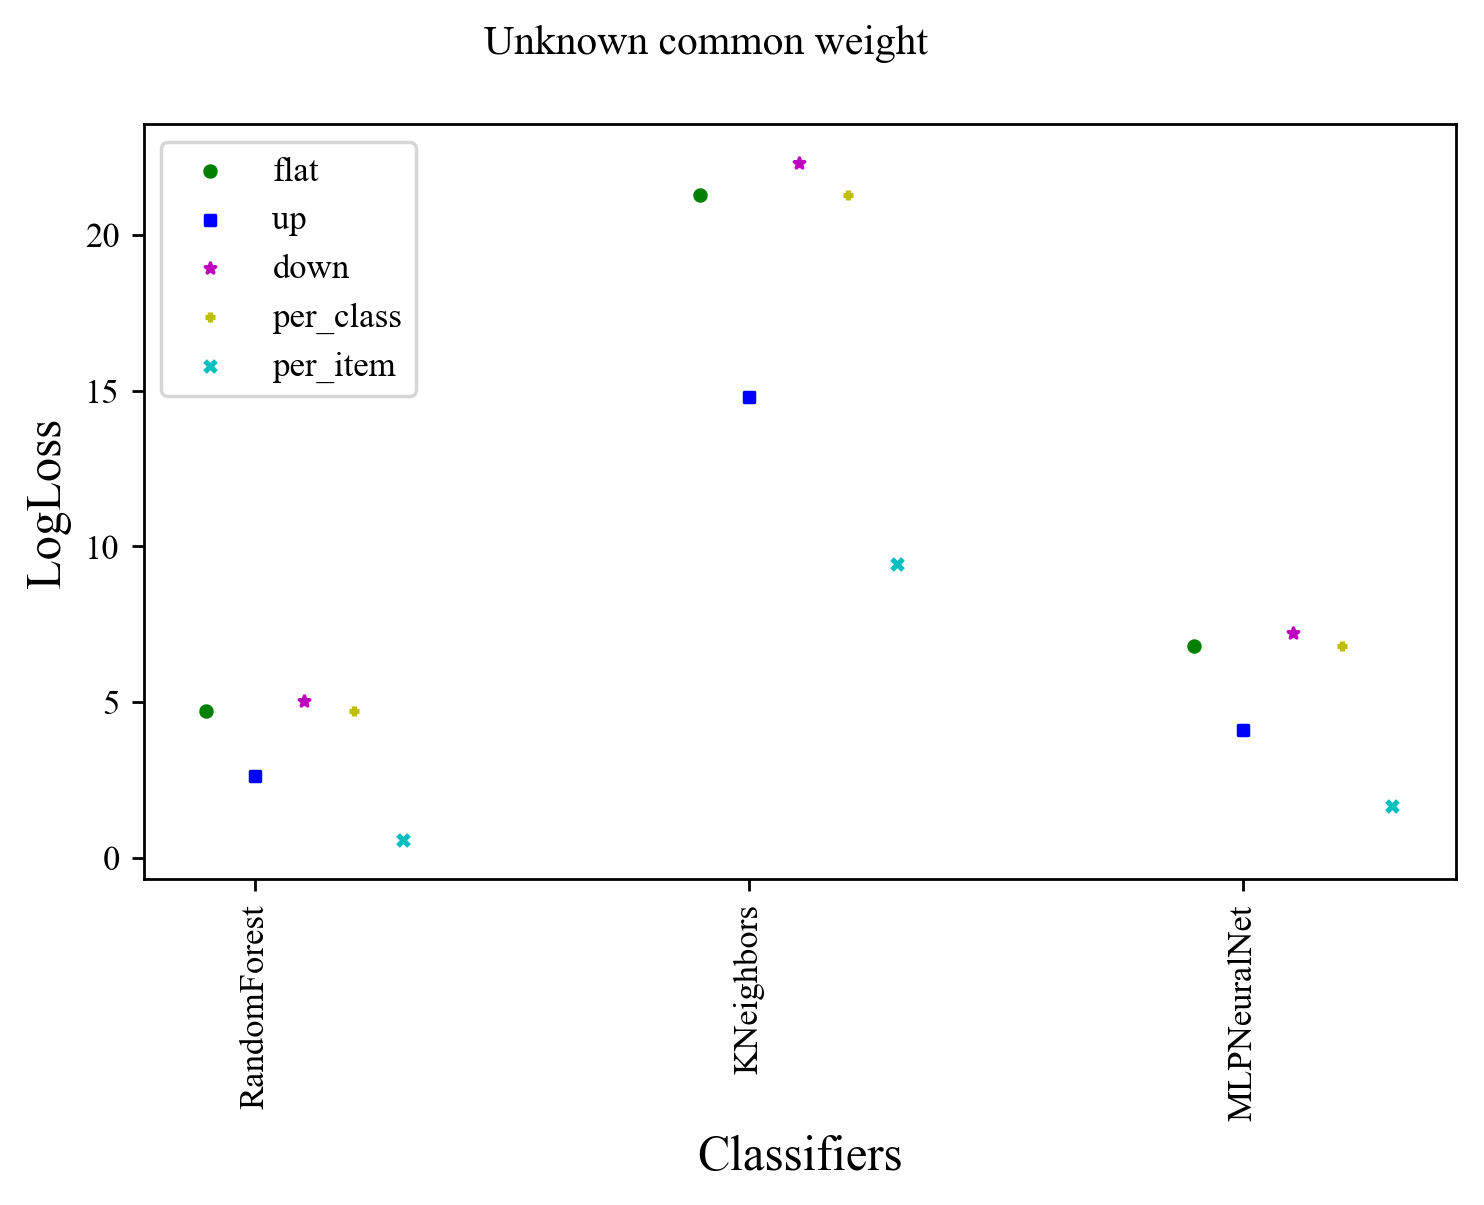
\includegraphics[width=0.5\textwidth]{./fig/systematic_Unknown_common.png}
		\caption{upweighting most common (best accuracy?)}
		\label{fig:systematic_common}
	\end{center}
\end{figure}

\begin{figure}
	\begin{center}
		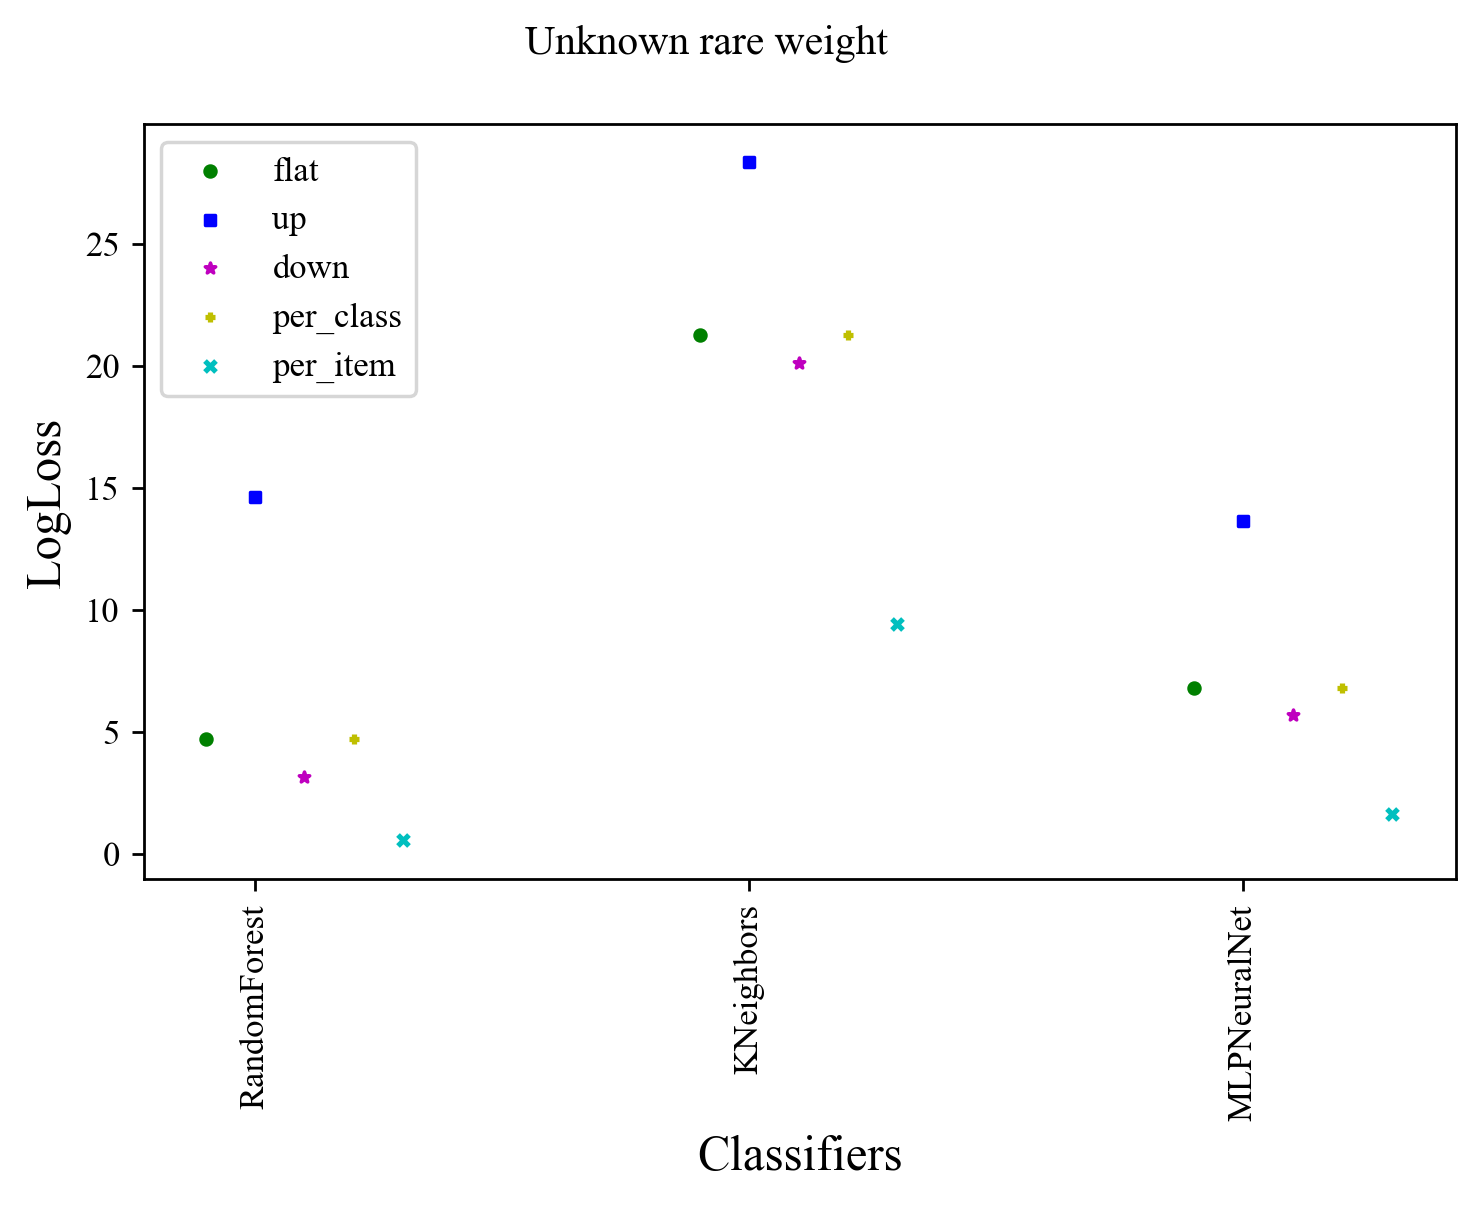
\includegraphics[width=0.5\textwidth]{./fig/systematic_Unknown_rare.png}
		\caption{upweighting least common (worst accuracy?)}
		\label{fig:systematic_rare}
	\end{center}
\end{figure}

\begin{figure}
	\begin{center}
		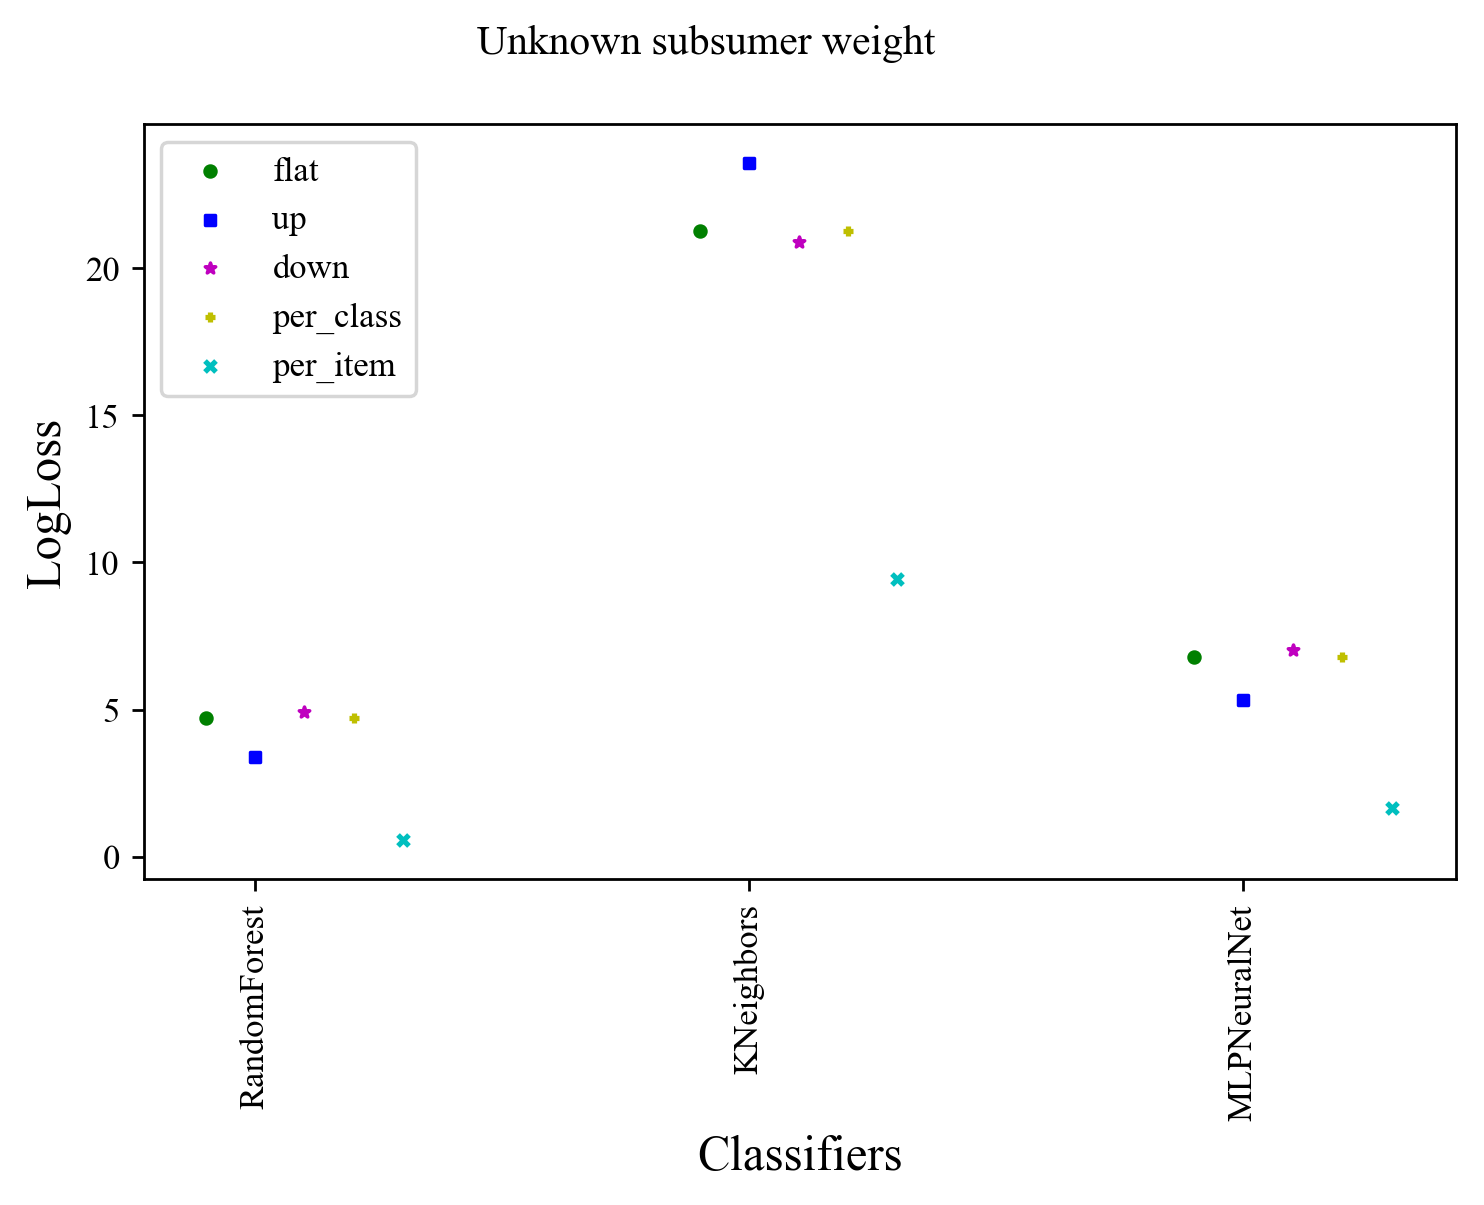
\includegraphics[width=0.5\textwidth]{./fig/systematic_Unknown_subsumer.png}
		\caption{upweighting class commonly misclassified as another class}
		\label{fig:systematic_subsumer}
	\end{center}
\end{figure}

\begin{figure}
	\begin{center}
		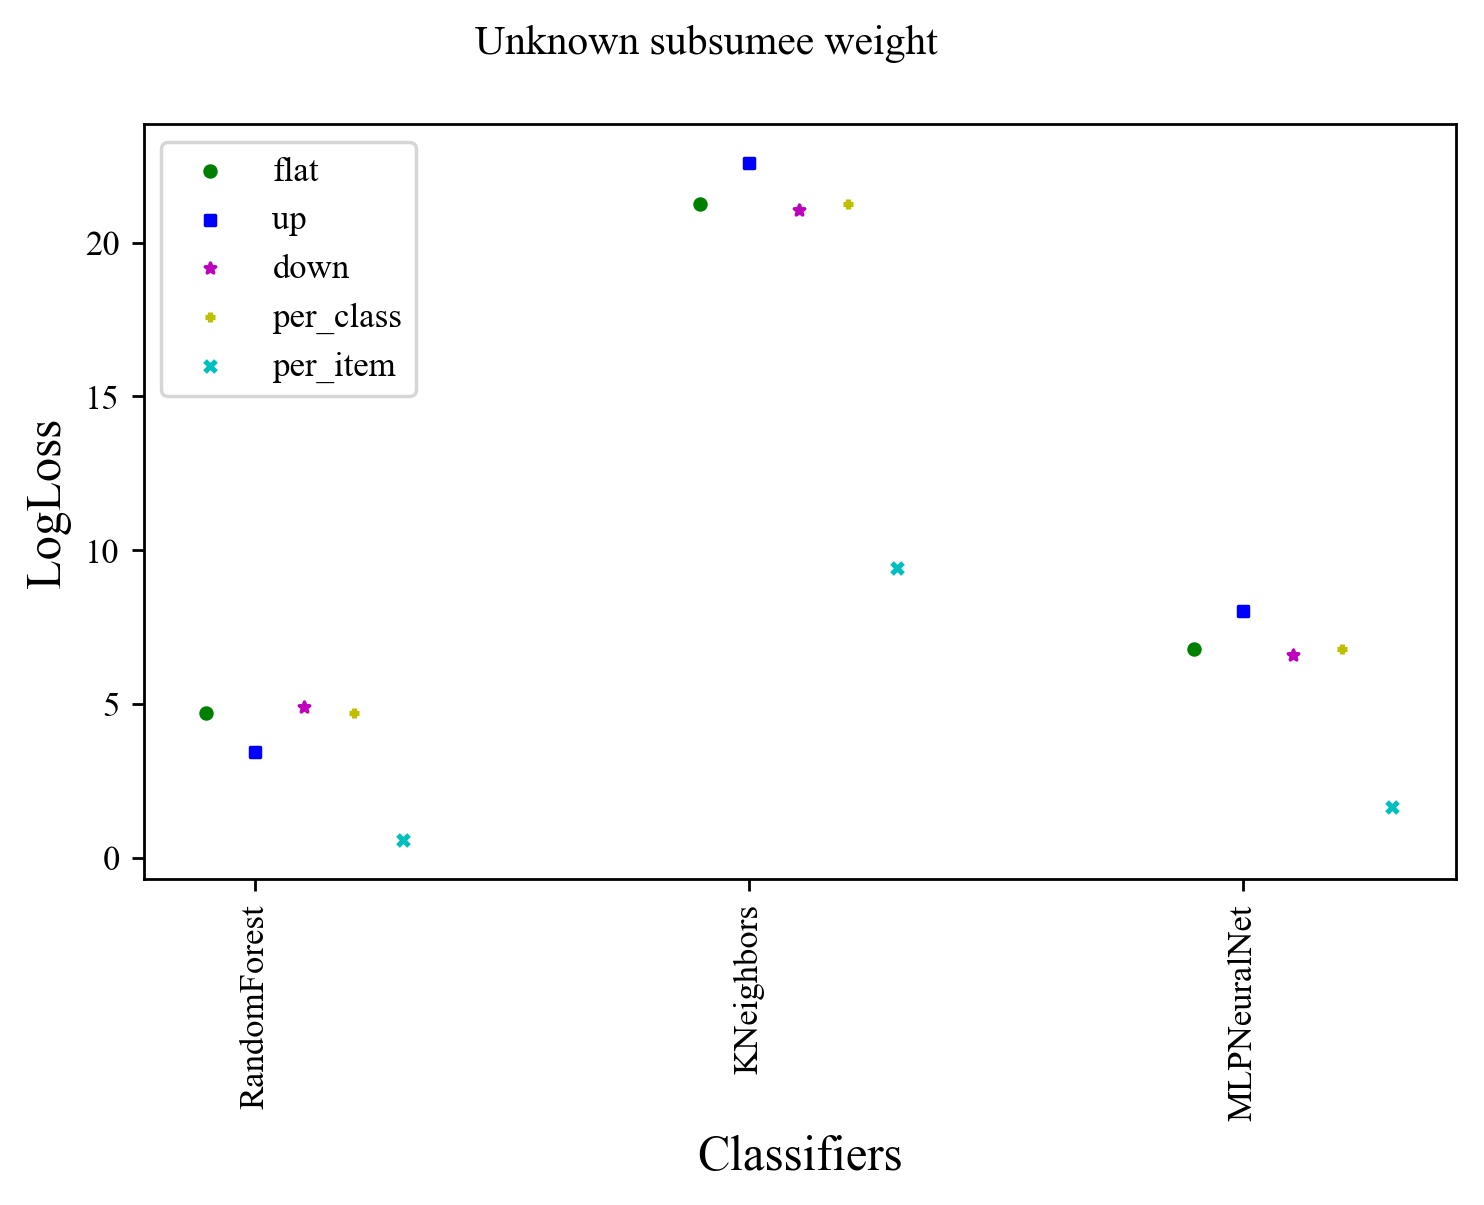
\includegraphics[width=0.5\textwidth]{./fig/systematic_Unknown_subsumee.png}
		\caption{upweighting class that a combination of other real classes are classified as}
		\label{fig:systematic_subsumee}
	\end{center}
\end{figure}

\begin{figure}
	\begin{center}
		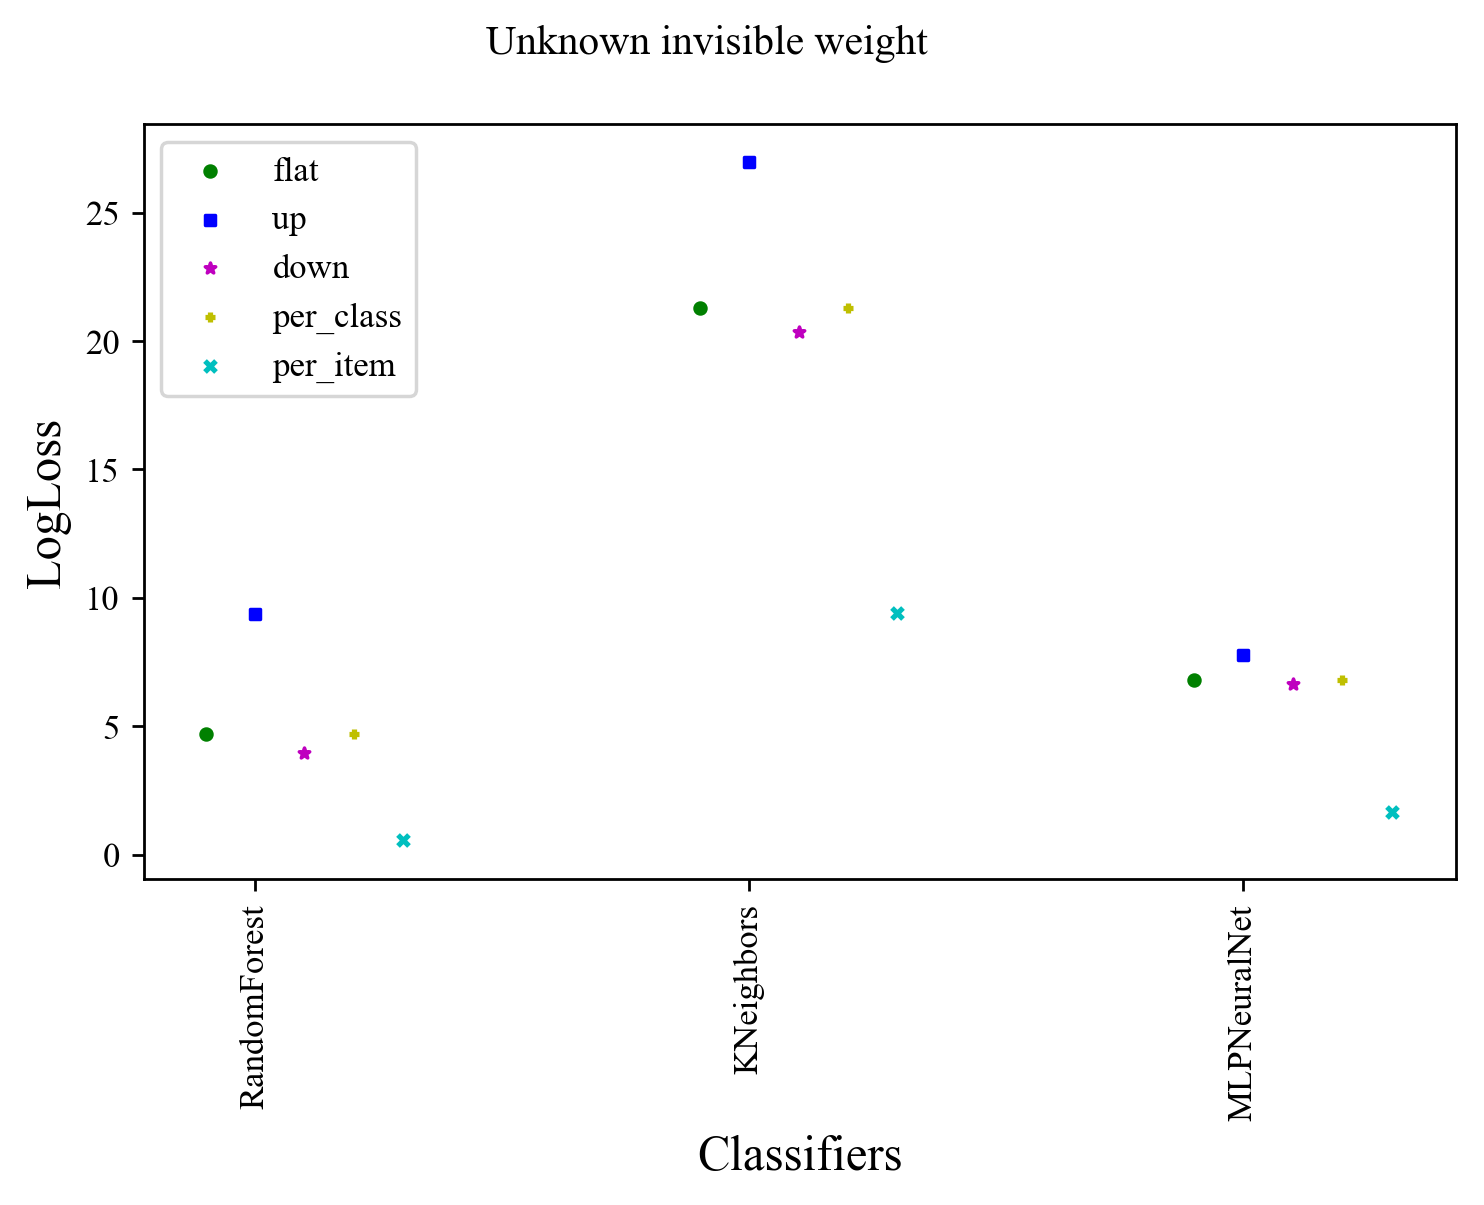
\includegraphics[width=0.5\textwidth]{./fig/systematic_Unknown_invisible.png}
		\caption{upweighting class that's totally missed}
		\label{fig:systematic_invisible}
	\end{center}
\end{figure}
